% Created by tikzDevice version 0.12.6 on 2024-09-26 13:54:17
% !TEX encoding = UTF-8 Unicode
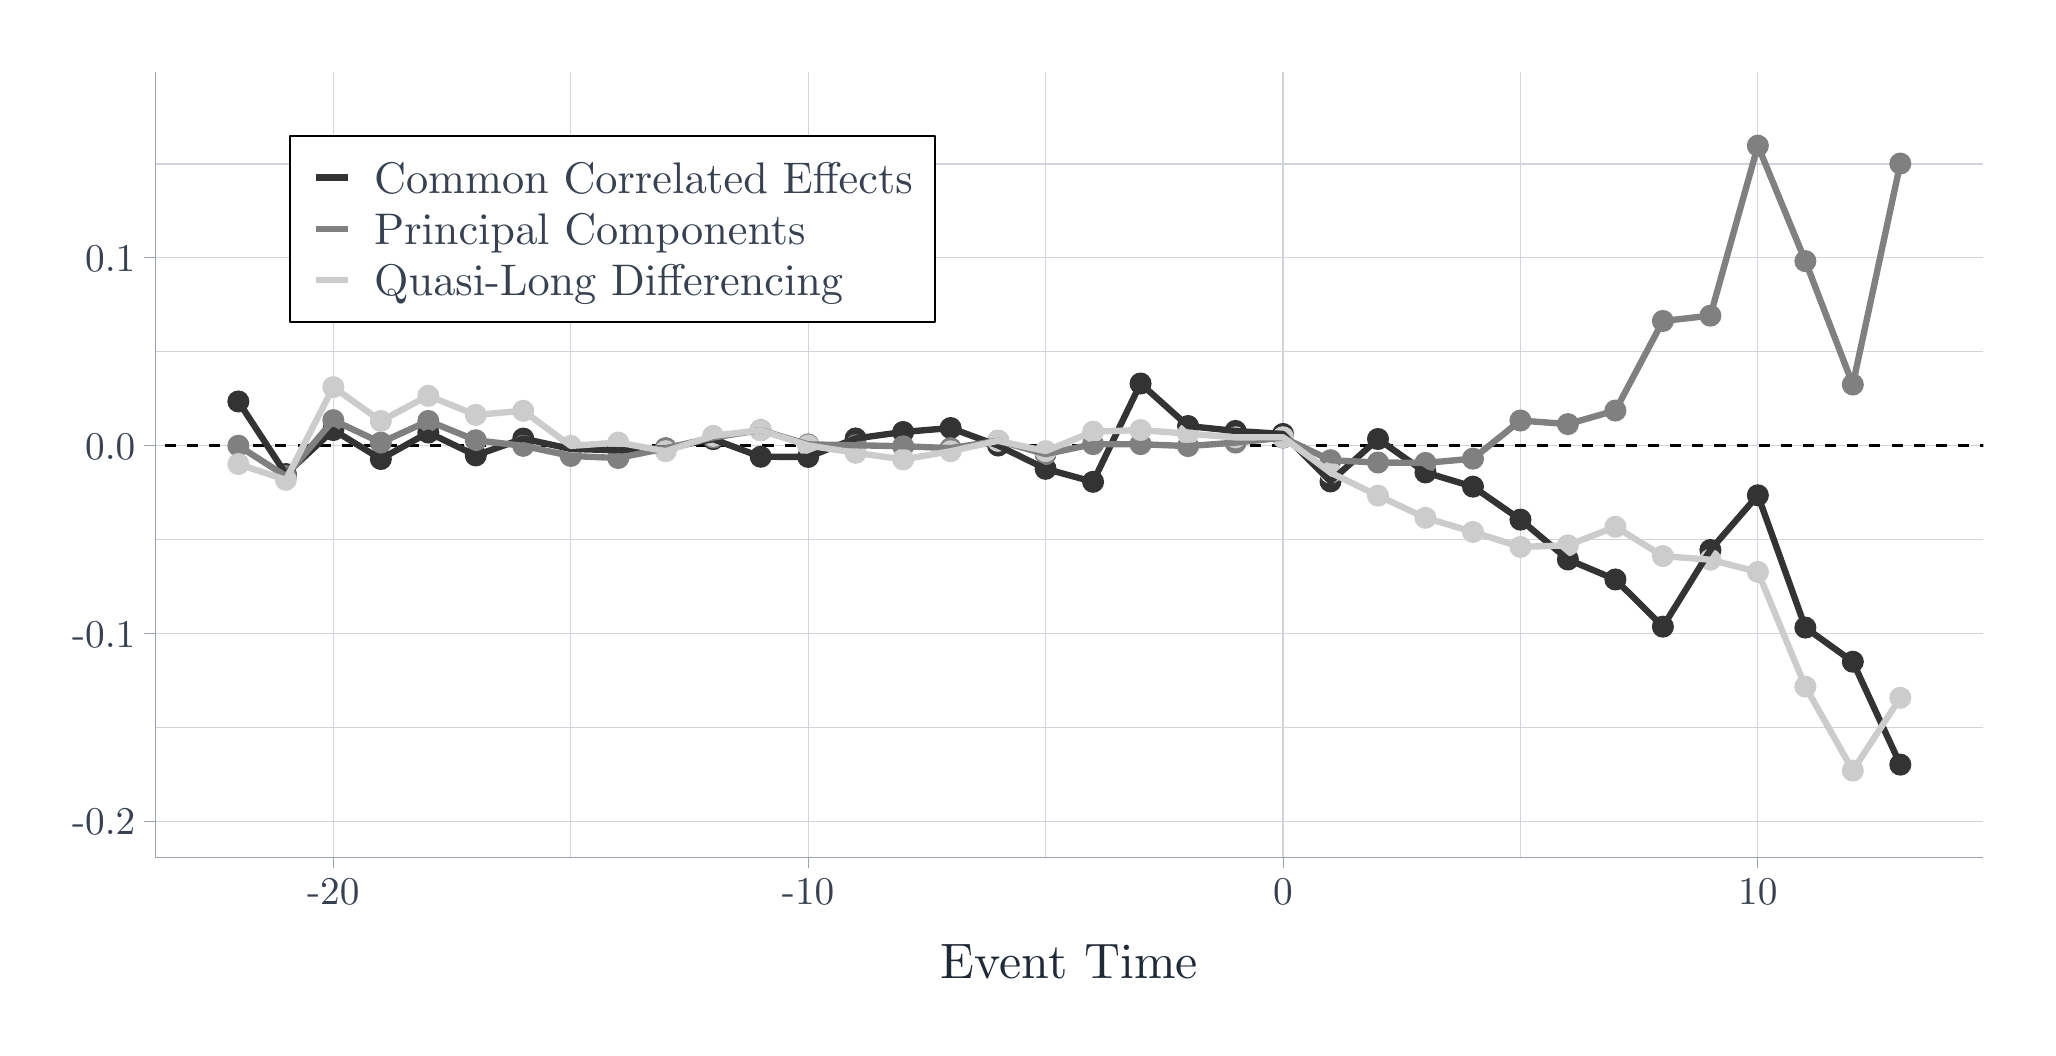
\begin{tikzpicture}[x=1pt,y=1pt]
\definecolor{fillColor}{RGB}{255,255,255}
\path[use as bounding box,fill=fillColor] (0,0) rectangle (722.70,361.35);
\begin{scope}
\path[clip] (  0.00,  0.00) rectangle (722.70,361.35);
\definecolor{drawColor}{RGB}{255,255,255}

\path[draw=drawColor,line width= 0.8pt,line join=round,line cap=round,fill=fillColor] (  0.00,  0.00) rectangle (722.70,361.35);
\end{scope}
\begin{scope}
\path[clip] ( 46.10, 61.65) rectangle (706.70,345.35);
\definecolor{drawColor}{RGB}{255,255,255}
\definecolor{fillColor}{RGB}{255,255,255}

\path[draw=drawColor,line width= 0.8pt,line join=round,line cap=round,fill=fillColor] ( 46.10, 61.65) rectangle (706.70,345.35);
\definecolor{drawColor}{RGB}{209,213,219}

\path[draw=drawColor,line width= 0.4pt,line join=round] ( 46.10,108.48) --
	(706.70,108.48);

\path[draw=drawColor,line width= 0.4pt,line join=round] ( 46.10,176.35) --
	(706.70,176.35);

\path[draw=drawColor,line width= 0.4pt,line join=round] ( 46.10,244.22) --
	(706.70,244.22);

\path[draw=drawColor,line width= 0.4pt,line join=round] ( 46.10,312.09) --
	(706.70,312.09);

\path[draw=drawColor,line width= 0.4pt,line join=round] (196.24, 61.65) --
	(196.24,345.35);

\path[draw=drawColor,line width= 0.4pt,line join=round] (367.82, 61.65) --
	(367.82,345.35);

\path[draw=drawColor,line width= 0.4pt,line join=round] (539.41, 61.65) --
	(539.41,345.35);

\path[draw=drawColor,line width= 0.4pt,line join=round] ( 46.10, 74.55) --
	(706.70, 74.55);

\path[draw=drawColor,line width= 0.4pt,line join=round] ( 46.10,142.42) --
	(706.70,142.42);

\path[draw=drawColor,line width= 0.4pt,line join=round] ( 46.10,210.29) --
	(706.70,210.29);

\path[draw=drawColor,line width= 0.4pt,line join=round] ( 46.10,278.16) --
	(706.70,278.16);

\path[draw=drawColor,line width= 0.4pt,line join=round] (110.45, 61.65) --
	(110.45,345.35);

\path[draw=drawColor,line width= 0.4pt,line join=round] (282.03, 61.65) --
	(282.03,345.35);

\path[draw=drawColor,line width= 0.4pt,line join=round] (453.61, 61.65) --
	(453.61,345.35);

\path[draw=drawColor,line width= 0.4pt,line join=round] (625.20, 61.65) --
	(625.20,345.35);
\definecolor{drawColor}{RGB}{0,0,0}

\path[draw=drawColor,line width= 0.9pt,dash pattern=on 4pt off 4pt ,line join=round] (-614.49,210.29) -- (1367.30,210.29);
\definecolor{drawColor}{gray}{0.20}
\definecolor{fillColor}{gray}{0.20}

\path[draw=drawColor,line width= 0.5pt,line join=round,line cap=round,fill=fillColor] ( 76.13,226.28) circle (  3.73);

\path[draw=drawColor,line width= 0.5pt,line join=round,line cap=round,fill=fillColor] ( 93.29,200.06) circle (  3.73);

\path[draw=drawColor,line width= 0.5pt,line join=round,line cap=round,fill=fillColor] (110.45,215.96) circle (  3.73);

\path[draw=drawColor,line width= 0.5pt,line join=round,line cap=round,fill=fillColor] (127.61,205.48) circle (  3.73);

\path[draw=drawColor,line width= 0.5pt,line join=round,line cap=round,fill=fillColor] (144.76,215.05) circle (  3.73);

\path[draw=drawColor,line width= 0.5pt,line join=round,line cap=round,fill=fillColor] (161.92,206.78) circle (  3.73);

\path[draw=drawColor,line width= 0.5pt,line join=round,line cap=round,fill=fillColor] (179.08,212.86) circle (  3.73);

\path[draw=drawColor,line width= 0.5pt,line join=round,line cap=round,fill=fillColor] (196.24,209.12) circle (  3.73);

\path[draw=drawColor,line width= 0.5pt,line join=round,line cap=round,fill=fillColor] (213.40,208.64) circle (  3.73);

\path[draw=drawColor,line width= 0.5pt,line join=round,line cap=round,fill=fillColor] (230.56,209.34) circle (  3.73);

\path[draw=drawColor,line width= 0.5pt,line join=round,line cap=round,fill=fillColor] (247.71,212.66) circle (  3.73);

\path[draw=drawColor,line width= 0.5pt,line join=round,line cap=round,fill=fillColor] (264.87,206.30) circle (  3.73);

\path[draw=drawColor,line width= 0.5pt,line join=round,line cap=round,fill=fillColor] (282.03,206.23) circle (  3.73);

\path[draw=drawColor,line width= 0.5pt,line join=round,line cap=round,fill=fillColor] (299.19,212.90) circle (  3.73);

\path[draw=drawColor,line width= 0.5pt,line join=round,line cap=round,fill=fillColor] (316.35,215.25) circle (  3.73);

\path[draw=drawColor,line width= 0.5pt,line join=round,line cap=round,fill=fillColor] (333.51,216.68) circle (  3.73);

\path[draw=drawColor,line width= 0.5pt,line join=round,line cap=round,fill=fillColor] (350.66,210.36) circle (  3.73);

\path[draw=drawColor,line width= 0.5pt,line join=round,line cap=round,fill=fillColor] (367.82,201.93) circle (  3.73);

\path[draw=drawColor,line width= 0.5pt,line join=round,line cap=round,fill=fillColor] (384.98,197.24) circle (  3.73);

\path[draw=drawColor,line width= 0.5pt,line join=round,line cap=round,fill=fillColor] (402.14,232.76) circle (  3.73);

\path[draw=drawColor,line width= 0.5pt,line join=round,line cap=round,fill=fillColor] (419.30,217.40) circle (  3.73);

\path[draw=drawColor,line width= 0.5pt,line join=round,line cap=round,fill=fillColor] (436.46,215.62) circle (  3.73);

\path[draw=drawColor,line width= 0.5pt,line join=round,line cap=round,fill=fillColor] (453.61,214.54) circle (  3.73);

\path[draw=drawColor,line width= 0.5pt,line join=round,line cap=round,fill=fillColor] (470.77,197.37) circle (  3.73);

\path[draw=drawColor,line width= 0.5pt,line join=round,line cap=round,fill=fillColor] (487.93,212.72) circle (  3.73);

\path[draw=drawColor,line width= 0.5pt,line join=round,line cap=round,fill=fillColor] (505.09,200.63) circle (  3.73);

\path[draw=drawColor,line width= 0.5pt,line join=round,line cap=round,fill=fillColor] (522.25,195.49) circle (  3.73);

\path[draw=drawColor,line width= 0.5pt,line join=round,line cap=round,fill=fillColor] (539.41,183.58) circle (  3.73);

\path[draw=drawColor,line width= 0.5pt,line join=round,line cap=round,fill=fillColor] (556.56,169.17) circle (  3.73);

\path[draw=drawColor,line width= 0.5pt,line join=round,line cap=round,fill=fillColor] (573.72,161.95) circle (  3.73);

\path[draw=drawColor,line width= 0.5pt,line join=round,line cap=round,fill=fillColor] (590.88,144.90) circle (  3.73);

\path[draw=drawColor,line width= 0.5pt,line join=round,line cap=round,fill=fillColor] (608.04,172.61) circle (  3.73);

\path[draw=drawColor,line width= 0.5pt,line join=round,line cap=round,fill=fillColor] (625.20,192.38) circle (  3.73);

\path[draw=drawColor,line width= 0.5pt,line join=round,line cap=round,fill=fillColor] (642.36,144.57) circle (  3.73);

\path[draw=drawColor,line width= 0.5pt,line join=round,line cap=round,fill=fillColor] (659.51,132.23) circle (  3.73);

\path[draw=drawColor,line width= 0.5pt,line join=round,line cap=round,fill=fillColor] (676.67, 95.05) circle (  3.73);
\definecolor{drawColor}{gray}{0.50}
\definecolor{fillColor}{gray}{0.50}

\path[draw=drawColor,line width= 0.5pt,line join=round,line cap=round,fill=fillColor] ( 76.13,210.28) circle (  3.73);

\path[draw=drawColor,line width= 0.5pt,line join=round,line cap=round,fill=fillColor] ( 93.29,199.29) circle (  3.73);

\path[draw=drawColor,line width= 0.5pt,line join=round,line cap=round,fill=fillColor] (110.45,219.51) circle (  3.73);

\path[draw=drawColor,line width= 0.5pt,line join=round,line cap=round,fill=fillColor] (127.61,211.41) circle (  3.73);

\path[draw=drawColor,line width= 0.5pt,line join=round,line cap=round,fill=fillColor] (144.76,219.24) circle (  3.73);

\path[draw=drawColor,line width= 0.5pt,line join=round,line cap=round,fill=fillColor] (161.92,212.27) circle (  3.73);

\path[draw=drawColor,line width= 0.5pt,line join=round,line cap=round,fill=fillColor] (179.08,210.24) circle (  3.73);

\path[draw=drawColor,line width= 0.5pt,line join=round,line cap=round,fill=fillColor] (196.24,206.59) circle (  3.73);

\path[draw=drawColor,line width= 0.5pt,line join=round,line cap=round,fill=fillColor] (213.40,205.84) circle (  3.73);

\path[draw=drawColor,line width= 0.5pt,line join=round,line cap=round,fill=fillColor] (230.56,209.35) circle (  3.73);

\path[draw=drawColor,line width= 0.5pt,line join=round,line cap=round,fill=fillColor] (247.71,213.27) circle (  3.73);

\path[draw=drawColor,line width= 0.5pt,line join=round,line cap=round,fill=fillColor] (264.87,215.91) circle (  3.73);

\path[draw=drawColor,line width= 0.5pt,line join=round,line cap=round,fill=fillColor] (282.03,210.77) circle (  3.73);

\path[draw=drawColor,line width= 0.5pt,line join=round,line cap=round,fill=fillColor] (299.19,210.45) circle (  3.73);

\path[draw=drawColor,line width= 0.5pt,line join=round,line cap=round,fill=fillColor] (316.35,210.11) circle (  3.73);

\path[draw=drawColor,line width= 0.5pt,line join=round,line cap=round,fill=fillColor] (333.51,209.41) circle (  3.73);

\path[draw=drawColor,line width= 0.5pt,line join=round,line cap=round,fill=fillColor] (350.66,212.08) circle (  3.73);

\path[draw=drawColor,line width= 0.5pt,line join=round,line cap=round,fill=fillColor] (367.82,207.25) circle (  3.73);

\path[draw=drawColor,line width= 0.5pt,line join=round,line cap=round,fill=fillColor] (384.98,210.84) circle (  3.73);

\path[draw=drawColor,line width= 0.5pt,line join=round,line cap=round,fill=fillColor] (402.14,210.84) circle (  3.73);

\path[draw=drawColor,line width= 0.5pt,line join=round,line cap=round,fill=fillColor] (419.30,210.15) circle (  3.73);

\path[draw=drawColor,line width= 0.5pt,line join=round,line cap=round,fill=fillColor] (436.46,211.41) circle (  3.73);

\path[draw=drawColor,line width= 0.5pt,line join=round,line cap=round,fill=fillColor] (453.61,213.22) circle (  3.73);

\path[draw=drawColor,line width= 0.5pt,line join=round,line cap=round,fill=fillColor] (470.77,205.05) circle (  3.73);

\path[draw=drawColor,line width= 0.5pt,line join=round,line cap=round,fill=fillColor] (487.93,204.22) circle (  3.73);

\path[draw=drawColor,line width= 0.5pt,line join=round,line cap=round,fill=fillColor] (505.09,204.07) circle (  3.73);

\path[draw=drawColor,line width= 0.5pt,line join=round,line cap=round,fill=fillColor] (522.25,205.61) circle (  3.73);

\path[draw=drawColor,line width= 0.5pt,line join=round,line cap=round,fill=fillColor] (539.41,219.39) circle (  3.73);

\path[draw=drawColor,line width= 0.5pt,line join=round,line cap=round,fill=fillColor] (556.56,218.10) circle (  3.73);

\path[draw=drawColor,line width= 0.5pt,line join=round,line cap=round,fill=fillColor] (573.72,223.00) circle (  3.73);

\path[draw=drawColor,line width= 0.5pt,line join=round,line cap=round,fill=fillColor] (590.88,255.36) circle (  3.73);

\path[draw=drawColor,line width= 0.5pt,line join=round,line cap=round,fill=fillColor] (608.04,257.28) circle (  3.73);

\path[draw=drawColor,line width= 0.5pt,line join=round,line cap=round,fill=fillColor] (625.20,318.70) circle (  3.73);

\path[draw=drawColor,line width= 0.5pt,line join=round,line cap=round,fill=fillColor] (642.36,276.98) circle (  3.73);

\path[draw=drawColor,line width= 0.5pt,line join=round,line cap=round,fill=fillColor] (659.51,232.40) circle (  3.73);

\path[draw=drawColor,line width= 0.5pt,line join=round,line cap=round,fill=fillColor] (676.67,312.24) circle (  3.73);
\definecolor{drawColor}{gray}{0.80}
\definecolor{fillColor}{gray}{0.80}

\path[draw=drawColor,line width= 0.5pt,line join=round,line cap=round,fill=fillColor] ( 76.13,203.67) circle (  3.73);

\path[draw=drawColor,line width= 0.5pt,line join=round,line cap=round,fill=fillColor] ( 93.29,197.96) circle (  3.73);

\path[draw=drawColor,line width= 0.5pt,line join=round,line cap=round,fill=fillColor] (110.45,231.47) circle (  3.73);

\path[draw=drawColor,line width= 0.5pt,line join=round,line cap=round,fill=fillColor] (127.61,219.21) circle (  3.73);

\path[draw=drawColor,line width= 0.5pt,line join=round,line cap=round,fill=fillColor] (144.76,228.33) circle (  3.73);

\path[draw=drawColor,line width= 0.5pt,line join=round,line cap=round,fill=fillColor] (161.92,221.43) circle (  3.73);

\path[draw=drawColor,line width= 0.5pt,line join=round,line cap=round,fill=fillColor] (179.08,222.91) circle (  3.73);

\path[draw=drawColor,line width= 0.5pt,line join=round,line cap=round,fill=fillColor] (196.24,210.21) circle (  3.73);

\path[draw=drawColor,line width= 0.5pt,line join=round,line cap=round,fill=fillColor] (213.40,211.43) circle (  3.73);

\path[draw=drawColor,line width= 0.5pt,line join=round,line cap=round,fill=fillColor] (230.56,208.31) circle (  3.73);

\path[draw=drawColor,line width= 0.5pt,line join=round,line cap=round,fill=fillColor] (247.71,213.86) circle (  3.73);

\path[draw=drawColor,line width= 0.5pt,line join=round,line cap=round,fill=fillColor] (264.87,215.87) circle (  3.73);

\path[draw=drawColor,line width= 0.5pt,line join=round,line cap=round,fill=fillColor] (282.03,210.37) circle (  3.73);

\path[draw=drawColor,line width= 0.5pt,line join=round,line cap=round,fill=fillColor] (299.19,207.72) circle (  3.73);

\path[draw=drawColor,line width= 0.5pt,line join=round,line cap=round,fill=fillColor] (316.35,205.33) circle (  3.73);

\path[draw=drawColor,line width= 0.5pt,line join=round,line cap=round,fill=fillColor] (333.51,208.28) circle (  3.73);

\path[draw=drawColor,line width= 0.5pt,line join=round,line cap=round,fill=fillColor] (350.66,212.07) circle (  3.73);

\path[draw=drawColor,line width= 0.5pt,line join=round,line cap=round,fill=fillColor] (367.82,208.34) circle (  3.73);

\path[draw=drawColor,line width= 0.5pt,line join=round,line cap=round,fill=fillColor] (384.98,215.37) circle (  3.73);

\path[draw=drawColor,line width= 0.5pt,line join=round,line cap=round,fill=fillColor] (402.14,215.96) circle (  3.73);

\path[draw=drawColor,line width= 0.5pt,line join=round,line cap=round,fill=fillColor] (419.30,214.63) circle (  3.73);

\path[draw=drawColor,line width= 0.5pt,line join=round,line cap=round,fill=fillColor] (436.46,213.30) circle (  3.73);

\path[draw=drawColor,line width= 0.5pt,line join=round,line cap=round,fill=fillColor] (453.61,213.35) circle (  3.73);

\path[draw=drawColor,line width= 0.5pt,line join=round,line cap=round,fill=fillColor] (470.77,200.57) circle (  3.73);

\path[draw=drawColor,line width= 0.5pt,line join=round,line cap=round,fill=fillColor] (487.93,192.24) circle (  3.73);

\path[draw=drawColor,line width= 0.5pt,line join=round,line cap=round,fill=fillColor] (505.09,184.23) circle (  3.73);

\path[draw=drawColor,line width= 0.5pt,line join=round,line cap=round,fill=fillColor] (522.25,179.13) circle (  3.73);

\path[draw=drawColor,line width= 0.5pt,line join=round,line cap=round,fill=fillColor] (539.41,173.71) circle (  3.73);

\path[draw=drawColor,line width= 0.5pt,line join=round,line cap=round,fill=fillColor] (556.56,174.30) circle (  3.73);

\path[draw=drawColor,line width= 0.5pt,line join=round,line cap=round,fill=fillColor] (573.72,180.99) circle (  3.73);

\path[draw=drawColor,line width= 0.5pt,line join=round,line cap=round,fill=fillColor] (590.88,170.41) circle (  3.73);

\path[draw=drawColor,line width= 0.5pt,line join=round,line cap=round,fill=fillColor] (608.04,169.10) circle (  3.73);

\path[draw=drawColor,line width= 0.5pt,line join=round,line cap=round,fill=fillColor] (625.20,164.66) circle (  3.73);

\path[draw=drawColor,line width= 0.5pt,line join=round,line cap=round,fill=fillColor] (642.36,123.23) circle (  3.73);

\path[draw=drawColor,line width= 0.5pt,line join=round,line cap=round,fill=fillColor] (659.51, 92.90) circle (  3.73);

\path[draw=drawColor,line width= 0.5pt,line join=round,line cap=round,fill=fillColor] (676.67,119.19) circle (  3.73);
\definecolor{drawColor}{gray}{0.20}

\path[draw=drawColor,line width= 2.3pt,line join=round] ( 76.13,226.28) --
	( 93.29,200.06) --
	(110.45,215.96) --
	(127.61,205.48) --
	(144.76,215.05) --
	(161.92,206.78) --
	(179.08,212.86) --
	(196.24,209.12) --
	(213.40,208.64) --
	(230.56,209.34) --
	(247.71,212.66) --
	(264.87,206.30) --
	(282.03,206.23) --
	(299.19,212.90) --
	(316.35,215.25) --
	(333.51,216.68) --
	(350.66,210.36) --
	(367.82,201.93) --
	(384.98,197.24) --
	(402.14,232.76) --
	(419.30,217.40) --
	(436.46,215.62) --
	(453.61,214.54) --
	(470.77,197.37) --
	(487.93,212.72) --
	(505.09,200.63) --
	(522.25,195.49) --
	(539.41,183.58) --
	(556.56,169.17) --
	(573.72,161.95) --
	(590.88,144.90) --
	(608.04,172.61) --
	(625.20,192.38) --
	(642.36,144.57) --
	(659.51,132.23) --
	(676.67, 95.05);
\definecolor{drawColor}{gray}{0.50}

\path[draw=drawColor,line width= 2.3pt,line join=round] ( 76.13,210.28) --
	( 93.29,199.29) --
	(110.45,219.51) --
	(127.61,211.41) --
	(144.76,219.24) --
	(161.92,212.27) --
	(179.08,210.24) --
	(196.24,206.59) --
	(213.40,205.84) --
	(230.56,209.35) --
	(247.71,213.27) --
	(264.87,215.91) --
	(282.03,210.77) --
	(299.19,210.45) --
	(316.35,210.11) --
	(333.51,209.41) --
	(350.66,212.08) --
	(367.82,207.25) --
	(384.98,210.84) --
	(402.14,210.84) --
	(419.30,210.15) --
	(436.46,211.41) --
	(453.61,213.22) --
	(470.77,205.05) --
	(487.93,204.22) --
	(505.09,204.07) --
	(522.25,205.61) --
	(539.41,219.39) --
	(556.56,218.10) --
	(573.72,223.00) --
	(590.88,255.36) --
	(608.04,257.28) --
	(625.20,318.70) --
	(642.36,276.98) --
	(659.51,232.40) --
	(676.67,312.24);
\definecolor{drawColor}{gray}{0.80}

\path[draw=drawColor,line width= 2.3pt,line join=round] ( 76.13,203.67) --
	( 93.29,197.96) --
	(110.45,231.47) --
	(127.61,219.21) --
	(144.76,228.33) --
	(161.92,221.43) --
	(179.08,222.91) --
	(196.24,210.21) --
	(213.40,211.43) --
	(230.56,208.31) --
	(247.71,213.86) --
	(264.87,215.87) --
	(282.03,210.37) --
	(299.19,207.72) --
	(316.35,205.33) --
	(333.51,208.28) --
	(350.66,212.07) --
	(367.82,208.34) --
	(384.98,215.37) --
	(402.14,215.96) --
	(419.30,214.63) --
	(436.46,213.30) --
	(453.61,213.35) --
	(470.77,200.57) --
	(487.93,192.24) --
	(505.09,184.23) --
	(522.25,179.13) --
	(539.41,173.71) --
	(556.56,174.30) --
	(573.72,180.99) --
	(590.88,170.41) --
	(608.04,169.10) --
	(625.20,164.66) --
	(642.36,123.23) --
	(659.51, 92.90) --
	(676.67,119.19);
\end{scope}
\begin{scope}
\path[clip] (  0.00,  0.00) rectangle (722.70,361.35);
\definecolor{drawColor}{RGB}{156,163,175}

\path[draw=drawColor,line width= 0.3pt,line join=round] ( 46.10, 61.65) --
	( 46.10,345.35);
\end{scope}
\begin{scope}
\path[clip] (  0.00,  0.00) rectangle (722.70,361.35);
\definecolor{drawColor}{RGB}{55,65,81}

\node[text=drawColor,anchor=base east,inner sep=0pt, outer sep=0pt, scale=  1.42] at ( 38.90, 69.65) {-0.2};

\node[text=drawColor,anchor=base east,inner sep=0pt, outer sep=0pt, scale=  1.42] at ( 38.90,137.52) {-0.1};

\node[text=drawColor,anchor=base east,inner sep=0pt, outer sep=0pt, scale=  1.42] at ( 38.90,205.39) {0.0};

\node[text=drawColor,anchor=base east,inner sep=0pt, outer sep=0pt, scale=  1.42] at ( 38.90,273.26) {0.1};
\end{scope}
\begin{scope}
\path[clip] (  0.00,  0.00) rectangle (722.70,361.35);
\definecolor{drawColor}{RGB}{156,163,175}

\path[draw=drawColor,line width= 0.3pt,line join=round] ( 42.10, 74.55) --
	( 46.10, 74.55);

\path[draw=drawColor,line width= 0.3pt,line join=round] ( 42.10,142.42) --
	( 46.10,142.42);

\path[draw=drawColor,line width= 0.3pt,line join=round] ( 42.10,210.29) --
	( 46.10,210.29);

\path[draw=drawColor,line width= 0.3pt,line join=round] ( 42.10,278.16) --
	( 46.10,278.16);
\end{scope}
\begin{scope}
\path[clip] (  0.00,  0.00) rectangle (722.70,361.35);
\definecolor{drawColor}{RGB}{156,163,175}

\path[draw=drawColor,line width= 0.3pt,line join=round] ( 46.10, 61.65) --
	(706.70, 61.65);
\end{scope}
\begin{scope}
\path[clip] (  0.00,  0.00) rectangle (722.70,361.35);
\definecolor{drawColor}{RGB}{156,163,175}

\path[draw=drawColor,line width= 0.3pt,line join=round] (110.45, 57.65) --
	(110.45, 61.65);

\path[draw=drawColor,line width= 0.3pt,line join=round] (282.03, 57.65) --
	(282.03, 61.65);

\path[draw=drawColor,line width= 0.3pt,line join=round] (453.61, 57.65) --
	(453.61, 61.65);

\path[draw=drawColor,line width= 0.3pt,line join=round] (625.20, 57.65) --
	(625.20, 61.65);
\end{scope}
\begin{scope}
\path[clip] (  0.00,  0.00) rectangle (722.70,361.35);
\definecolor{drawColor}{RGB}{55,65,81}

\node[text=drawColor,anchor=base,inner sep=0pt, outer sep=0pt, scale=  1.42] at (110.45, 44.66) {-20};

\node[text=drawColor,anchor=base,inner sep=0pt, outer sep=0pt, scale=  1.42] at (282.03, 44.66) {-10};

\node[text=drawColor,anchor=base,inner sep=0pt, outer sep=0pt, scale=  1.42] at (453.61, 44.66) {0};

\node[text=drawColor,anchor=base,inner sep=0pt, outer sep=0pt, scale=  1.42] at (625.20, 44.66) {10};
\end{scope}
\begin{scope}
\path[clip] (  0.00,  0.00) rectangle (722.70,361.35);
\definecolor{drawColor}{RGB}{31,41,55}

\node[text=drawColor,anchor=base,inner sep=0pt, outer sep=0pt, scale=  1.80] at (376.40, 17.75) {Event Time};
\end{scope}
\begin{scope}
\path[clip] (  0.00,  0.00) rectangle (722.70,361.35);
\definecolor{drawColor}{RGB}{0,0,0}
\definecolor{fillColor}{RGB}{255,255,255}

\path[draw=drawColor,line width= 0.6pt,line join=round,line cap=round,fill=fillColor] ( 94.74,254.93) rectangle (327.77,322.29);
\end{scope}
\begin{scope}
\path[clip] (  0.00,  0.00) rectangle (722.70,361.35);
\definecolor{drawColor}{RGB}{255,255,255}
\definecolor{fillColor}{RGB}{255,255,255}

\path[draw=drawColor,line width= 0.8pt,line join=round,line cap=round,fill=fillColor] (102.74,299.84) rectangle (117.19,314.29);
\end{scope}
\begin{scope}
\path[clip] (  0.00,  0.00) rectangle (722.70,361.35);
\definecolor{drawColor}{gray}{0.20}
\definecolor{fillColor}{gray}{0.20}

\path[draw=drawColor,line width= 0.5pt,line join=round,line cap=round,fill=fillColor] (109.97,307.06) circle (  0.52);
\end{scope}
\begin{scope}
\path[clip] (  0.00,  0.00) rectangle (722.70,361.35);
\definecolor{drawColor}{gray}{0.20}

\path[draw=drawColor,line width= 2.5pt,line join=round] (104.18,307.06) -- (115.75,307.06);
\end{scope}
\begin{scope}
\path[clip] (  0.00,  0.00) rectangle (722.70,361.35);
\definecolor{drawColor}{RGB}{255,255,255}
\definecolor{fillColor}{RGB}{255,255,255}

\path[draw=drawColor,line width= 0.8pt,line join=round,line cap=round,fill=fillColor] (102.74,281.38) rectangle (117.19,295.84);
\end{scope}
\begin{scope}
\path[clip] (  0.00,  0.00) rectangle (722.70,361.35);
\definecolor{drawColor}{gray}{0.50}
\definecolor{fillColor}{gray}{0.50}

\path[draw=drawColor,line width= 0.5pt,line join=round,line cap=round,fill=fillColor] (109.97,288.61) circle (  0.52);
\end{scope}
\begin{scope}
\path[clip] (  0.00,  0.00) rectangle (722.70,361.35);
\definecolor{drawColor}{gray}{0.50}

\path[draw=drawColor,line width= 2.5pt,line join=round] (104.18,288.61) -- (115.75,288.61);
\end{scope}
\begin{scope}
\path[clip] (  0.00,  0.00) rectangle (722.70,361.35);
\definecolor{drawColor}{RGB}{255,255,255}
\definecolor{fillColor}{RGB}{255,255,255}

\path[draw=drawColor,line width= 0.8pt,line join=round,line cap=round,fill=fillColor] (102.74,262.93) rectangle (117.19,277.38);
\end{scope}
\begin{scope}
\path[clip] (  0.00,  0.00) rectangle (722.70,361.35);
\definecolor{drawColor}{gray}{0.80}
\definecolor{fillColor}{gray}{0.80}

\path[draw=drawColor,line width= 0.5pt,line join=round,line cap=round,fill=fillColor] (109.97,270.16) circle (  0.52);
\end{scope}
\begin{scope}
\path[clip] (  0.00,  0.00) rectangle (722.70,361.35);
\definecolor{drawColor}{gray}{0.80}

\path[draw=drawColor,line width= 2.5pt,line join=round] (104.18,270.16) -- (115.75,270.16);
\end{scope}
\begin{scope}
\path[clip] (  0.00,  0.00) rectangle (722.70,361.35);
\definecolor{drawColor}{RGB}{55,65,81}

\node[text=drawColor,anchor=base west,inner sep=0pt, outer sep=0pt, scale=  1.60] at (125.19,301.56) {Common Correlated Effects};
\end{scope}
\begin{scope}
\path[clip] (  0.00,  0.00) rectangle (722.70,361.35);
\definecolor{drawColor}{RGB}{55,65,81}

\node[text=drawColor,anchor=base west,inner sep=0pt, outer sep=0pt, scale=  1.60] at (125.19,283.10) {Principal Components};
\end{scope}
\begin{scope}
\path[clip] (  0.00,  0.00) rectangle (722.70,361.35);
\definecolor{drawColor}{RGB}{55,65,81}

\node[text=drawColor,anchor=base west,inner sep=0pt, outer sep=0pt, scale=  1.60] at (125.19,264.65) {Quasi-Long Differencing};
\end{scope}
\end{tikzpicture}
